\documentclass{article}


% if you need to pass options to natbib, use, e.g.:
\PassOptionsToPackage{numbers, compress}{natbib}
% before loading neurips_2023


% ready for submission
%\usepackage{neurips_2023}


% to compile a preprint version, e.g., for submission to arXiv, add add the
% [preprint] option:
% \usepackage[preprint]{neurips_2023}


% to compile a camera-ready version, add the [final] option, e.g.:
\usepackage[final]{neurips_2023}


% to avoid loading the natbib package, add option nonatbib:
% \usepackage[nonatbib]{neurips_2023}


\usepackage[utf8]{inputenc} % allow utf-8 input
\usepackage[T1]{fontenc}    % use 8-bit T1 fonts
\usepackage{hyperref}       % hyperlinks
\usepackage{url}            % simple URL typesetting
\usepackage{booktabs}       % professional-quality tables
\usepackage{amsfonts}       % blackboard math symbols
\usepackage{nicefrac}       % compact symbols for 1/2, etc.
\usepackage{microtype}      % microtypography
\usepackage{xcolor}         % colors

% added packages
\usepackage{amsmath}
\usepackage{amssymb}
\usepackage{dsfont}
\usepackage{graphicx}
\usepackage{tikz}


\title{A Deep Learning approach to detect sleep state - Midterm Report}


% The \author macro works with any number of authors. There are two commands
% used to separate the names and addresses of multiple authors: \And and \AND.
%
% Using \And between authors leaves it to LaTeX to determine where to break the
% lines. Using \AND forces a line break at that point. So, if LaTeX puts 3 of 4
% authors names on the first line, and the last on the second line, try using
% \AND instead of \And before the third author name.


\author{%
  Armando Bringas \\
  2023490306 \\
  International Student \\
  Tecnológico de Monterrey \\
  Querétaro, México \\
  % \texttt{armandobringas10@mails.tsinghua.edu.cn} \\
  % examples of more authors
  \And
  Alexis Guerrero \\
  2023480366 \\
  International Student \\
  Universidad de Chile \\
  Santiago de Chile, Chile \\
  % \texttt{guerreromontea10@mails.tsinghua.edu.cn} \\
}


\begin{document}


\maketitle





\begin{abstract}
This investigation proposes a project that utilizes deep learning techniques to address the complex task of detecting sleep states using accelerometer data from wrist-worn devices. This research include a review and critical evaluation of various deep learning architectures, comparing them with other machine learning strategies to determine the most effective approach. With an initial focus on examining state-of-the-art methods, central to this proposal is the development of a deep learning solution for analyzing and predicting time-series data from these wrist-worn devices to accurately identify sleep states. The overarching aim is to implement a reliable predictive model that significantly enhances the precision and dependability of sleep state classification using data from wearable technology.
\end{abstract}


\section{Introduction}

This paper presents a project proposal rooted in the practical application of a Kaggle competition, aimed at addressing a challenge in pediatric health and neuroscience: the identification of sleep states in children through wrist-worn accelerometer data. The competition serves as a catalyst for innovation, prompting the development of a sophisticated machine learning model capable of discerning the subtle onset of various sleep states and periods of wakefulness with precision.

The significance of this project lies in its potential to deepen our understanding of sleep and to provide further insights into its importance. For instance, understanding how environmental factors influence sleep, mood, and behavior can aid in formulating personalized strategies tailored to the unique needs of each child \cite{child-mind-institute-detect-sleep-states}. Furthermore, the outcomes of this project could enable researchers to undertake more comprehensive, large-scale sleep studies across a variety of populations and contexts, which could yield even more valuable information about sleep \cite{child-mind-institute-detect-sleep-states}.

\section{Literature Review}

For this type of problem, a Machine Learning approach based on Random Forest has proven effective in detecting sleep-wake states, non-wear versus wear, and sleep stage classification \cite{Sundararajan2021}. An initial attempt was made using a Residual Neural Network (RNN), specifically a ResNet initialized with a Glorot uniform initializer and employing LeakyReLU activations \cite{Sundararajan2021}. However, when testing this approach with the Amsterdam dataset, which consists of data collected from 114 individuals recruited by the VU University Medical Center in Amsterdam, The Netherlands \cite{teLindert2020}, it was observed that the Random Forest approach outperformed the ResNet heuristic. Notably, the ResNet had difficulties with wake state prediction \cite{Sundararajan2021}. However, it is important to remark that most the used data was collected with the GENActiv accelerometer brand, it should be consider future studies to assess model transferability across other accelerometer brands \cite{Sundararajan2021}.

We explored another approach that analyzes data from the VU University Medical Center in Amsterdam, The Netherlands \cite{teLindert2020}. Unlike machine learning methods, this study employed Latent Class Analysis (LCA), a statistical method rather than a machine learning or deep learning technique. LCA, commonly used in social, psychological, and behavioral sciences, identifies latent classes within populations sharing common characteristics \cite{qing2023}. In their study, LCA was utilized to differentiate subtypes of sleep misperception among individuals using data from actigraphy and sleep diaries from the people in their studies \cite{teLindert2020}. Sleep misperception, in this context, is the discrepancy between subjectively perceived and objectively measured sleep, crucial for understanding disorders like Insomnia Disorder \cite{teLindert2020}. This study, focusing on a statistical categorical approach to classify sleep misperception, falls outside our scope.

Also, it is important to note that the analyzed information for sleep state detection can come from different types of devices, from example from an optical plethysmography and accelerometer signals \cite{Beattie_2017} \cite{Fedorin2019}, depending on the research. Specifically, there are cases in which the data is extracted from accelerometers among other types of sensors. Therefore, the methods utilized in each case serve as a baseline for their respective projects, this means that couldn't be possible a suitable that generalize over the data coming from different sources.

Understanding the clinical implications of devices employed for sleep state detection is crucial. Accelerometry is frequently utilized as a cost-effective method for assessing sleep states. However, it appears that traditional machine learning algorithms may have limitations in accuracy, particularly in patients with insomnia \cite{Sundararajan2021}. There exists both an opportunity and a growing interest in refining these algorithms by enhancing the accuracy of accelerometry could transform it into a more clinically valuable tool, enabling the measurement of sleep and wakefulness over prolonged periods \cite{Sundararajan2021}.

Despite evidence suggesting that classical methods, such as Support Vector Machines, effectively detect sleep states and may outperform Deep Learning methods in specific scenarios with data from actigraph devices that recorded signals using a microelectromechanical system (MEMS) accelerometer \cite{teLindert2020}, similar to the GENActiv accelerometer \cite{Sundararajan2021}, were analyzed., we explored alternative approaches. Our investigation revealed the deployment of Deep Learning and other Machine Learning models for detecting sleep states from various source signals. These include electrocardiography (ECG), which measures the heart's electrical activity in combination of respiratory and movement signals \cite{Stuburic2020}, or electroencephalogram (EEG), employing electrodes on the scalp to monitor brain electrical signals \cite{Sekkal2022}. Other sources involve a combination of optical plethysmography and accelerometer signals \cite{Beattie_2017} \cite{Fedorin2019}, and more complex inputs like multi-channel polysomnogram (PSG) \cite{Li2021}. PSG encompasses diverse physiological continuous-time signals from multiple sensors, including EEG, electrooculography (EOG) for eye movement, electromyography (EMG) for muscle contractions, and monitors for respiration and body oxygen levels \cite{Li2021}.

Although the different source signals, overally, they shared in common the complexity, high-dimensionality, noise and temporo-spatial dependency structure of these data types that make them suitable for analysis using deep learning models with their respective challenges \cite{thomas2018}. A potential challenge could yield with working with raw signals introduced with the network without doing feature extraction \cite{Stuburic2020}. From the work of \cite{michielli2019} they compare different methods and algorithms based on data from heart rate and wrist actigraphy, but they did low-level and mid-level feature extraction before introducing to the network, the best results was obtained from a Long Short-Term Memory LSTM network for 2-class classification with an accuracy of 83.56\% \cite{michielli2019}.

A Long Short-Term Memory network (LSTM) is a specialized type of Recurrent Neural Network (RNN). It's important to note that RNNs are a natural choice for time-series forecasting and prediction \cite{Aggarwal2018}. LSTM enhances the RNN architecture by modifying the recurrence conditions of how the hidden states are propagated \cite{Aggarwal2018}. Additionally, it addresses the challenges of vanishing and exploding gradients, which are critical issues in neural network training \cite{Aggarwal2018, michielli2019}.

In their research, Sekkal et al. \cite{Sekkal2022} utilized a LSTM network for analyzing the Physionet Sleep-EDF Database, containing 153 polysomnograms (PSGs) from two-night recordings. Feature extraction was performed to refine the data within the PSG signals. The study's relevance stems from its comparison of classical machine learning techniques with deep learning approaches, notably focusing on LSTM due to its proficiency in identifying temporal relationships between sleep stages \cite{Sekkal2022}. In their bi-directional LSTM classifier implementation, an accuracy of 87.8\% was achieved on the PSG (Fpz-Cz + Pz-Oz + EOG) classifier. Contrasting this, Fraiwan \& Alkhodari \cite{fraiwan2020} reported a peak accuracy of 97.1\% using a bi-directional LSTM with a single channel. However, their training set showed significant class imbalance, with the 'awake' stage constituting 68\% of the epochs. This imbalance likely skewed the classifier's performance, favoring the more prevalent sleep stage.

The bi-directional LSTM classifier model, referenced in the studies by Sekkal et al. \cite{Sekkal2022} and Fraiwan \& Alkhodari \cite{fraiwan2020}, represents an enhancement of the standard LSTM. This variant eliminates the one-step truncation inherent in the original LSTM design. Bidirectional training possesses an architectural advantage over unidirectional training if used
to classify phonemes \cite{Graves2005}, it incorporates a comprehensive error gradient calculation, enabling training through standard backpropagation through time (BPTT) \cite{Staudemeyer2019}.

Is important to remark that Fiorillo et al. \cite{Fiorillo2019} present a systematic and comprehensive review of deep learning algorithms applied to sleep scoring. The paper thoroughly examines the latest applications and compares them to other methodologies, it concluded that deep learning methods offer numerous advantages. Notably, these algorithms can be applied directly to raw data in comparison with other approaches that involved feature extraction \cite{Stuburic2020} \cite{michielli2019}, therefore requiring minimal artifact removal. Furthermore, they are capable of unveiling hidden information that traditional feature-based approaches might overlook.

Finally, in the work of \cite{Stuburic2020} they implemented a LSTM architecture with the raw signals from EEG without any prior feature extraction. The preprocessing involved reducing noise and smoothing the signal using a median filter and, in some cases, applying signal flipping or baseline subtraction. LSTM were designed to learn features directly from these raw, preprocessed signals without any feature extraction step, they achieved an accuracy of 80\% in 5-class classification.

To address our particular challenge, we propose initially implementing an LSTM architecture without feature extraction. This approach is selected based on revisited literature that emphasizes its effectiveness in capturing temporal dependencies in sequential data, a key characteristic of our problem domain. Subsequent stages of our research will involve evaluating the performance of this model and discussing potential enhancements. These may include the integration of feature extraction techniques or the exploration of other Deep Learning architectures, as needed.


\section{A Machine Learning and Deep Learning approaches}

The global objective is to apply a Deep Learning architecture to the dataset provided by \cite{child-mind-institute-detect-sleep-states}. Our primary motivation emanates from the efficacy of deep learning methodologies in the realm of time series analysis, with a particular focus on the 'Detect Sleep States' dataset from the Child Mind Institute \cite{child-mind-institute-detect-sleep-states}. Furthermore, we aim to employ both Long Short-Term Memory (LSTM) networks and Random Forests as part of our methodology. The dual utilization of these approaches seeks to explore the comparative advantages and complexities that each method might offer in the context of sleep state detection. Finally, upon completion of the implementation phase, a comprehensive benchmarking analysis will be conducted to compare and contrast the performance of the LSTM and Random Forest models, providing a deeper insight into their respective strenghts and limitations.


\subsection{Data}

 As shown in Table \ref{fig:accelerometerdata_dataframe}, the dataset consists of approximately 500 multi-day recordings from wrist-mounted accelerometers. The accelerometer data in the dataset was processed using R with the GGIR package \cite{Migueles2019GGIR}. The recordings are labeled with two event types: 'onset', indicating the start of sleep, and 'wakeup', marking its end. The primary objective is to identify these two events within the accelerometer data series, this primarily represents a binary classification task. 

  \begin{table*}[ht]
    \centering
    \caption{Random sample series from the dataset}
    \begin{tabular}{|c|c|c|c|c|c|}
        \hline
        \textbf{series\_id} & \textbf{step} & \textbf{timestamp} & \textbf{anglez} & \textbf{enmo} & \textbf{awake} \\
        \hline
        fa149c3c4bde & 96695 & 2018-09-05T09:17:55-0400 & -35.085 & 0.0153 & 0 \\
        aa81faa78747 & 173071 & 2018-03-09T17:22:35-0500 & -21.0547 & 0.0504 & 0 \\
        9c91c546e095 & 325646 & 2018-06-12T08:47:10-0400 & -15.5015 & 0.0261 & 0 \\
        601559e1777d & 94646 & 2019-03-27T22:57:10-0400 & 5.6094 & 0.0000 & 1 \\
        188d4b7cd28b & 353126 & 2017-11-29T02:42:10-0500 & -37.105 & 0.0158 & 0 \\
        c289c8a823e0 & 596500 & 2018-07-11T22:58:20-0400 & -25.187 & 0.0085 & 0 \\
        0402a003dae9 & 315686 & 2019-01-05T19:12:10-0500 & -22.3541 & 0.0235 & 1 \\
        c38707ef76df & 321529 & 2018-06-03T01:04:05-0400 & -5.1726 & 0.1138 & 0 \\
        b7188813d58a & 125675 & 2018-10-11T18:32:55-0400 & 26.7438 & 0.0016 & 1 \\
        ece2561f07e9 & 424534 & 2017-09-02T01:52:50-0400 & -68.6974 & 0.0000 & 0 \\
        \hline
    \end{tabular}
    \label{fig:accelerometerdata_dataframe}
\end{table*}

As shown in Figures \ref{fig:accelerometerdata_series-038441c925bb_anglez}, \ref{fig:accelerometerdata_series-038441c925bb_enmo}, the data represents series of continuous recording of the accelerometer data for a single subject spanning many days, where we can find:

 \begin{itemize}
  \item \texttt{series\_id}: Unique identifier for each accelerometer series.
    \item \texttt{step}: An integer timestep for each observation within a series. It is uniqute within a series
  \item \texttt{event}: The type of event, whether onset [0] or wakeup [1].
  \item \texttt{timestamp}: A corresponding datetime in ISO 8601 format: \%Y-\%m-\%dT\%H:\%M:\%S\%z.
  \item \texttt{anglez}: As calculated and described by the GGIR package, z-angle is a metric derived from individual accelerometer components that is commonly used in sleep detection, and refers to the angle of the arm relative to the vertical axis of the body \cite{Migueles2019GGIR}.
  \item \texttt{enmo}: As calculated and described by the GGIR package, ENMO is the Euclidean Norm Minus One of all accelerometer signals, with negative values rounded to zero. While no standard measure of acceleration exists in this space, this is one of the several commonly computed features \cite{Migueles2019GGIR}.
\end{itemize}

 \begin{figure*}[ht]
    \centering
    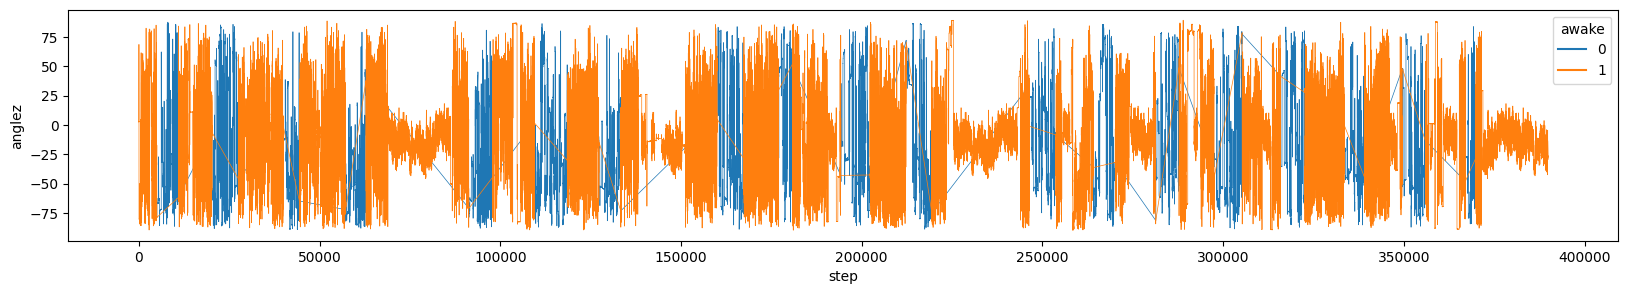
\includegraphics[width=1\linewidth]{figures/038441c925bb_anglez.png}
    \caption{Accelerometer training data. Plot of \texttt{step} againts \texttt{anglez} showing \texttt{event} state}
    \label{fig:accelerometerdata_series-038441c925bb_anglez}
\end{figure*}



 \begin{figure*}[ht]
    \centering
    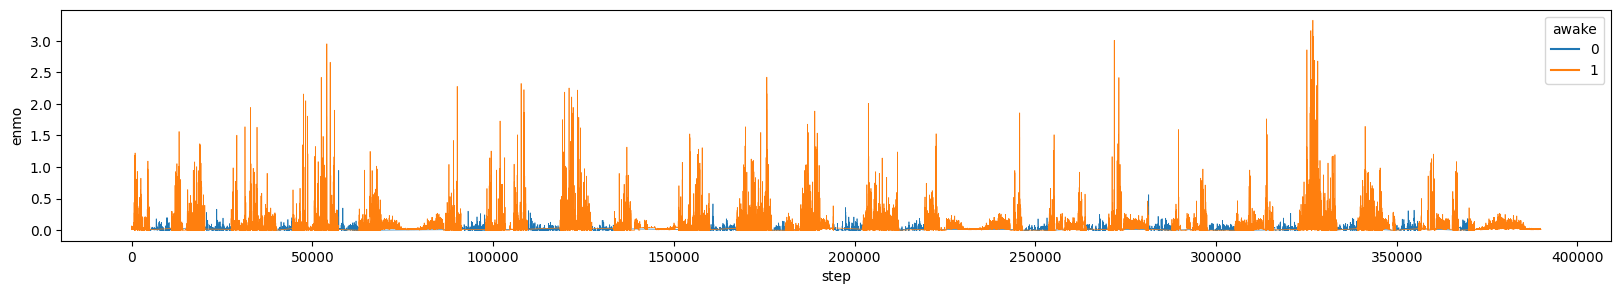
\includegraphics[width=1\linewidth]{figures/038441c925bb_enmo.png}
    \caption{Accelerometer training data. Plot of \texttt{step} againts \texttt{enmo} showing \texttt{event} state}
    \label{fig:accelerometerdata_series-038441c925bb_enmo}
\end{figure*}


    
 \subsection{Model}

 \subsection{Random Forest}

Alongside the implementation of the LSTM model, a Random Forest model will be incorporated to explore an alternative approach in this study. The selection of this model was predicated upon a comprehensive review of the literature conducted during the preliminary phases of this project. As demonstrated in prior cases, Random Forest has exhibited commendable performance and accuracy in the detection of sleep stages, rendering it a suitable method for comparison with the primary model to be developed in our project, namely LSTM.

The Random Forest model is initialized with a predetermined number of $100$ estimators (\textit{n\textunderscore estimators}) and a minimum leaf sample size (\textit{min\textunderscore sample\textunderscore leaf}) set to $300$. These initial values are chosen for the purpose of assessing the model's efficiency and will be subject to subsequent adjustments based on its performance. Given the substantial volume of data in this scenario, it is anticipated that the minimum leaf sample size will remain unchanged, whereas the number of estimators will likely need to be increased to optimize performance.

To ensure reproducibility, a seed is fixed by setting the \textit{random\textunderscore state} to a value generated randomly by using the random module in python. This measure allows the code to generate consistent results when executed with the same seed in the future. Additionally, the \textit{n\textunderscore jobs} parameter from the scikit-learn library is configured with a value of $-1$, enabling the utilization of all available processors on the device running the code.

The model implementation is configured with an iterative approach to allow certain values in the initialization process to vary. This enables the acquisition of a greater variety of results in a controlled manner. Specifically, the parameters ``n\textunderscore estimators'' and ``random\textunderscore state'' are subject to variation. At the onset of the iterations, a random value between $1$ and $500$ is set as the seed for ``random \textunderscore state'' and this value remains constant for a total of 3 iterations. The value for ``n\textunderscore estimators'' starts at $100$, and with each subsequent iteration, it increases to $200$ and $300$, respectively. Subsequently, in the next iteration, the entire process is repeated. This approach generates sets of results with different seeds, and for each seed, a set of results is obtained for varying values of ``n\textunderscore estimators''. This methodology provides a diverse range of results for subsequent metric evaluation of the model, offering insights into its performance under different ``random\textunderscore state'' seeds and ``n\textunderscore estimators'' values.

Let us delve into a more detailed examination of this iterative process. Let $\mathcal{X}_{RF}$ be a generalization of the input data received by the Random Forest model. The model is implemented through iterations, let $\mathcal{Y}_{RF_i}$ be a generalization of the model output data at the $i$th iteration. See the diagram below:

\begin{center}
  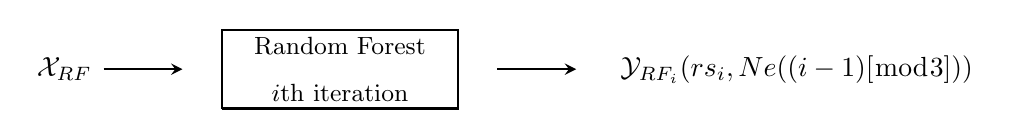
\begin{tikzpicture}
    \node at (0,0) (XRF) {$\mathcal{X}_{RF}$} ;
    \draw[thick, -stealth] (0.5,0) -- (1.5,0) ;
    \draw[thick] (2,-0.5) -- (5,-0.5) -- (5,0.5) -- (2,0.5) -- (2,-0.5) ;
    \node at (3.5,0.3) {\small{Random Forest}} ;
    \node at (3.5,-0.3) {\small{$i$th iteration}} ;
    \draw[thick, -stealth] (5.5,0) -- (6.5,0) ;
    \node at (9.3,0) (YRF) {$\mathcal{Y}_{RF_i}(rs_i,Ne((i-1)[\bmod{3}]))$} ;
  \end{tikzpicture}  
\end{center}

Where ($rs_i$,$Ne((i-1)[\bmod{3}])$) is the pair of elements that characterizes the output data at the $i$th iteration, formed by the random\textunderscore state and n\textunderscore estimators values respectively. Both elements are described as follows:

Let $R_s = \{rs_1, rs_2, \ldots , rs_{N/3}\} \subset \mathds{Z}$ be the set of all different random\textunderscore states values.

And $I = \{1, \ldots , N\} \subset \mathds{Z}$ the set of values taken by the iteration.

Notice that $rs_j \in R_s$ is an arbitary value in $R_s$.

In particular $rs_j \in [1,500] \forall j \in \mathds{N}$ such that $1 \leq j \leq \frac{N}{3}$.

If $rs_i$ is the random\textunderscore state value for the $i$th iteration, then:

\begin{equation*}
  rs_i = rs_j \ \forall i \in I \text{ such that } i \leq 3j \wedge i > 3(j-1)
\end{equation*}

On another hand; $Ne((i-1)[\bmod{3}])$ is a function that gives the n\textunderscore estimators value for each iteration, such that:

\[
Ne((i-1)[\bmod{3}]) =
\begin{cases}
  100 \text{, if } (i-1)[\bmod{3}] = 0 \\
  200 \text{, if } (i-1)[\bmod{3}] = 1 \\
  300 \text{, if } (i-1)[\bmod{3}] = 2
\end{cases}
\]

Finally, the generalization for the model output data in each iteration, along with irs characterization (that relies on the random\textunderscore states and n\textunderscore estimators values) is given by:

\begin{equation*}
  \mathcal{Y}_{RF_i}(rs_i,Ne((i-1)[\bmod{3}]))
\end{equation*}

This representation allow us to have a variety of data, which is treated after in the model evaluation phase. Mainly, we can separate it by the random\textunderscore state value or the n\textunderscore estimators one. Each classification is presented as follows:

By the random\textunderscore state value:

\begin{gather*}
  \mathcal{Y}_{RF_1} = \{(rs_i,Ne((i-1)[\bmod{3})) \in \mathcal{Y}_{RF_i}, rs_i = rs_1\} \\
  \mathcal{Y}_{RF_2} = \{(rs_i,Ne((i-1)[\bmod{3})) \in \mathcal{Y}_{RF_i}, rs_i = rs_2\} \\
  \vdots \\
  \mathcal{Y}_{RF_{N/3}} = \{(rs_i,Ne((i-1)[\bmod{3})) \in \mathcal{Y}_{RF_i}, rs_i = rs_{N/3}\}  
\end{gather*}

By the n\textunderscore estimators value:

\begin{gather*}
  \mathcal{Y}_{100} = \{(rs_i,Ne((i-1)[\bmod{3})) \in \mathcal{Y}_{RF_i}, Ne((i-1)[\bmod{3}]) = 0\} \\
  \mathcal{Y}_{200} = \{(rs_i,Ne((i-1)[\bmod{3})) \in \mathcal{Y}_{RF_i}, Ne((i-1)[\bmod{3}]) = 1\} \\
  \mathcal{Y}_{300} = \{(rs_i,Ne((i-1)[\bmod{3})) \in \mathcal{Y}_{RF_i}, Ne((i-1)[\bmod{3}]) = 2\}
\end{gather*}

\subsubsection{LSTM - Long Short Term Memory}

We are planning to implement an architecture that incorporates an LSTM cell into our sequence of input data. In this cell architecture, the intermediate variables \( \overline{i}, \overline{f}, \overline{o} \), corresponding to the \textit{input}, \textit{forget}, and \textit{output} gates, play crucial roles in updating the cell and hidden states. The determination of the hidden state vector \( \overline{h}^{(k)}_{t} \) and the cell state vector \( \overline{c}^{(k)}_{t} \) is a multi-step process that starts by computing the intermediate variables, followed by the computation of the hidden states from these intermediates \cite{Aggarwal2018}. The updates are as follows:

\vspace{0.5em}

\textbf{[Setting up intermediates]}
\begin{align*}
\begin{matrix}
\text{Input Gate:} \\
\text{Forget Gate:} \\
\text{Output Gate:} \\
\text{New C.-State:} \\
\end{matrix} &\begin{bmatrix}
\overline{i} \\ 
\overline{f} \\
\overline{o} \\
\overline{c} \\
\end{bmatrix} =
\begin{bmatrix}
\text{sigm} \\
\text{sigm} \\
\text{sigm} \\
\tanh \\
\end{bmatrix} W^{(k)}
\begin{bmatrix}
h_{t}^{(k-1)} \\
h_{t-1}^{(k)}
\end{bmatrix}
\end{align*}

\textbf{[Selectively forget and add to long-term memory]}

\begin{equation*}
\begin{aligned}
    \overline{c}^{(k)}_{t} = \overline{f} \odot \overline{c}^{(k)}_{t-1} + \overline{i} \odot \overline{c} \\
\end{aligned}
\end{equation*}

\textbf{[Selectively leak long-term memory to hidden state]}

\begin{equation*}
\begin{aligned}
    \overline{h}^{(k)}_{t} &= o_t \odot \tanh(\overline{c}^{(k)}_{t})
\end{aligned}
\end{equation*}

Our neural network architecture employs an LSTM to incorporate the classifications of previous inputs into the current sample's classification. This approach is suitable to looking back to inform the present, a method particularly suited for cyclical patterns like sleep stages \cite{Stuburic2020}, which recur throughout the night. Therefore, LSTMs, with their recurrent nature, could be an ideal choice for this type of cyclic temporal problems.

As shown in Figure \ref{fig:neuralnetwork} 
We are proposing a starting neural network architecture with the following blocks where consists of a LSTM layer of 64 units, ideal for processing sequences by capturing dependencies from prior inputs. This is followed by a Dense layer, the size of which matches the number of classification categories in your problem, in this case for our binary classification problem \(n_classes = 2\). The final component is a softmax activation function, applied to convert the output into a probability distribution across the predicted classes. 

\begin{figure}[h]
  \centering
  \[
  \xrightarrow{\text{input}} \boxed{\text{LSTM} (64)} \rightarrow \boxed{\text{Dense} (n_{\text{classes}})} \xrightarrow{\text{softmax}}
  \]
  \caption{Neural Network for accelerometer data classification}
  \label{fig:neuralnetwork}
\end{figure}

Let's explore in more detail the procedural aspects illustrated in the above figure. To achieve this objective, we will begin by generalizing the input data that the LSTM model is expected to receive. Let $\mathcal{X}_{input}$ be a seet with all the input data, such that:

Considering an arbitrary number of temporal sequences $N$, we have $\mathcal{X}_{input} = \{\mathcal{X}_1, \mathcal{X}_2, \ldots , \mathcal{X}_N \}$

Where each temporal sequence is the set of data with equal \textit{series\textunderscore id} value. Considering an arbitrary number of events for the temporal sequence, $M$, we have: $\mathcal{X}_i = \{\mathcal{X}_{i1}, \mathcal{X}_{i2}, \ldots , \mathcal{X}_{iM}\}, \forall i \in \mathds{N}, 1 \leq i \leq N$

Notice that $\mathcal{X}_{ij}, \forall j \in \mathds{N}, 1 \leq j \leq M$ is an arbitrary temporal sequence, with an arbitary number of characteristics, $n$, such that $\mathcal{X}_{ij} \in \mathds{R}^n, n \in \mathds{N}$, described as $\mathcal{X}_{ij} = (x_{ij1}, x_{ij2}, \ldots , x_{ijn})$

Aditionally, notice that $x_{ijk}, \forall k \in \mathds{N}, 1 \leq k \leq n$ is the $k$th characteristic from the $j$th event in the $i$th temporal sequence from the set of input data $\mathcal{X}_{input}$

This information can be express in another way using tensors, such that the input data set is a tensor $X_{input}$ such that $X_{input} \in \mathds{R}^{N \times M \times n}$ with each individual element denoted by $X_{i,j,k}$.

During the feature engineering phase, three functions are applied to an arbitrary temporal sequence $\mathcal{X}_i$, denoted by $f_1$, $f_2$ and $f_3$. These functions introduce a determined number of characteristics to the events in the temporal sequence. We can make a generalization of the output in this process through a function composition, as follows:


Let $\mathcal{XF}_i$ be the output from the feature engineering phase;
\begin{equation*}
  \mathcal{XF}_i = f_3(f_2(f_1(\mathcal{X}_i)))
\end{equation*}

A new set is created during the Data Preprocessing phase, $DP = \{ (\mathcal{XF}_{i,j},\mathcal{Y}_{i,j}) \}_{j=1}^M$, where $\mathcal{Y}_{i,j}$ is the objective vector with the respectively classe. As this is a binary classification problem, $\mathcal{Y}_{i,j} \in \mathds{R}$, with values of $0$ or $1$. The output of this phase will be denoted as $DPO = \{ (\mathcal{XF}'_{i,j},\mathcal{Y}'_{i,j}) \}_{j=1}^M$

Both $\mathcal{XF}'_{i,j}$ and $\mathcal{Y}'_{i,j}$ elements are separated during the split data section.

Let $\mathcal{X}' = \{ \mathcal{XF}'_{i,j} \}_{j=1}^M$ and $\mathcal{Y}'' = \{ \mathcal{Y}'_{i,j} \}_{j=1}^M$ be sets for the characteristics vectors and objetive variables respectively. Both sets are represented as tensors as follows:

\begin{equation*}
  \mathcal{X}' = (M,n); \mathcal{X}' \in \mathds{R}^{M \times n} \& \mathcal{Y}' = (M); \mathcal{Y}' \in \mathds{Z}^M
\end{equation*}

Still in the data splitting phase, distinct sets are generated for both the training data $T$ and the validation data $V$. These sets can be succinctly represented using tensors as follows:

For the training data; $(\mathcal{X}'_t,\mathcal{Y}'_t)$, where $\mathcal{X}'_t \in \mathds{R}^{M_{Train}\times n}$ and $\mathcal{Y}'_t \in \mathds{Z}^{M_{Train}}$. Here $M_{Train}$ is the fraction of data asociated with the training process.

For the validation data; $(\mathcal{X}'_v, \mathcal{Y}'_v)$ where $\mathcal{X}'_v \in \mathds{R}^{M_{Validation} \times n}$ and $\mathcal{Y}'_v \in \mathds{Z}^{M_{Validation}}$. Here $M_{Validation}$ is the fraction of data associated with the validation process. The data is aggregated and organized during the data loader phase, prior to its entry into the LSTM model as previously elucidated at the outset of this section.

After the Dense phase, an outpur vector $O$ is generated. Due to the nature of this classification (binary), $O \in \mathds{R}^2$, such that:

\begin{equation*}
  O = (o_1, o_2)
\end{equation*}

Where $o_1, o_2 \in \mathds{R}$ each characterizing one of the two classes within this binary classification. Subsequently, a softmax function is applied to generate a probability distribution from the output vector, as detailed below:

For each $o_i, i = 1,2$ value of the output vector $O$ the softmax function is presented as follows:

\begin{equation*}
  \text{softmax}(o_i) = \frac{e^{o_i}}{\sum_{h=1}^G e^{o_h}}
\end{equation*}

In this aprticular case, and taking $\text{softmax}(o_i) = sm(o_i)$ we have $sm(O) = (sm(o_1), sm(o_2))$

Where $sm(o_i) \in [0,1], \forall i, i =1,2 \wedge \sum_{h=1}^2 sum(o_h) = 1$

Finally, is important to check if the impact to work directly with raw signals, the effects of the noise and the implications of not doing feature extraction do not affect performance in the training of the model. Subsequently, with the results of the first trials we might plan work more in data pre-processing if needed or even transition to more complex architectures. Other point of consideration is that one of the common problems is that the time-series sequences can be extremely long and therefore can be certain limitations with its performance \cite{Aggarwal2018}.

\subsection{Evaluation}

To evaluate model classification, three factors will be taken into account; the average precision ($AP$), the sensitivity or recall ($SN$) and the specificity ($SPC$). Each one is described as follows:

\subsubsection{Average Precision}

Let $\mathcal{X}$ be a vector with all the inputs of the model, from $x_1$ to $x_N$, supossing an arbitrary quantity of $N$ elements of data, with $N \in \mathds{N}$. Let $\mathcal{Y}$ be a vector with all the model outputs, from $y_1$ to $y_N$ under the same previous assumptions. Also, let $\mathcal{W}$ be a vector with all the labels for the model, represented from $w_1$ to $w_N$. Then, we have:

\begin{gather}
  \text{Inputs} \ \mathcal{X} = (x_1, \ldots, x_N)^\intercal \\
  \text{Outputs} \ \mathcal{Y} = (y_1, \ldots, y_N)^\intercal \\
  \text{Labels} \ \mathcal{W} = (w_1, \ldots, w_N)^\intercal 
\end{gather}

The average precision function, compares the quantity of succesful predictions with the total quantity of data. We define this function as follows:

\begin{equation*}
AP = \frac{1}{N} \sum_{i=1}^{N}{\mathcal{C}(w_i,y_i)}
\end{equation*}

Where $\mathcal{C}(w_i,y_i)$ is a function such that:

\[
\mathcal{C}(w_i,y_i) =
\begin{cases}
  1 \text{ if } w_i = y_i \forall i \in \mathds{N}, 1 \leq i \leq N\\
  0 \text{ if } w_i \neq y_i \forall i \in \mathds{N}, 1 \leq i \leq N
\end{cases}
\]

Then, doing a redefinition of this function as:

\begin{equation*}
APF(\mathcal{W}, \mathcal{Y}) = \frac{1}{N} A 1_N
\end{equation*}

Where $A$ is a matrix of $1 \times N$ which each of its elements described by $\omega_i$, where $ \omega_i = \mathcal{C}(w_i,y_i), \forall i \in \mathds{N}, 1 \leq i \leq N$ and $1_N$ is a matrix of $N \times 1$ with all of its elements being $1$. Finally, we can define our average precision function as:

\begin{gather}
  APF(\mathcal{W}, \mathcal{Y}) = \frac{1}{N} A 1_N \\
  APF(\mathcal{W}, \mathcal{Y}) = \frac{1}{N} (\omega_1, \ldots, \omega_N) (1, \ldots, 1)^\intercal 
\end{gather}

\subsubsection{Specificity and Sensitivity/Recall}


To evaluate model classification, predictions that align with the ground truth and exceed the threshold are labeled as True Positives (TP). Predictions that do not match are labeled as False Positives (FP), while ground truths without a corresponding prediction are labeled as False Negatives (FN). Where,

\[
\text{Score}(x) = 
\begin{cases} 
\text{TP} & \text{if }x \text{ matched and } x > \text{thresh.} \\
\text{FP} & \text{if }x \text{ unmatched pred.} \\
\text{FN} & \text{if }x \text{ unmatched truth} \\
\text{TN} & \text{otherwise}
\end{cases}
\]

We can make two measurements with this information, being the first; specificity, the rate of true positives and the second; sensitivity or recall, the rate or true negatives. Each ones is defined below with its corresponding notation ($SPC$ and $SN$)

\begin{gather}
  SPC = \frac{TP}{TP + FN} \\
  SN = \frac{TN}{TN + FP}
\end{gather}

\subsubsection{Final evaluation of model classification}

With $APF$, $SPC$ and $SN$ the average precision function, the specificity and the sensitivity or recall, as defined before. And with $\alpha$, $\beta$, $\gamma$ values that weight each metric, we have our final expression as described here:

\begin{equation*}
\text{Model evaluation } = \alpha APF + \beta SPC + \gamma SN 
\end{equation*}

\vspace{.5em}



\section{Results}

\begin{table}[h]
    \centering
    \caption{Random Forest Confusion Matrix}
    \label{tab:random_forest_confusion_matrix}
    \begin{tabular}{lcc}
        \hline
        \textbf{Actual / Predicted} & \textbf{Predicted Negative} & \textbf{Predicted Positive} \\
        \hline
        \textbf{Actual Negative} & 786677 (31.38\%) & 56959 (2.27\%) \\
        \textbf{Actual Positive} & 70514 (2.81\%) & 1592674 (63.53\%) \\
        \hline
    \end{tabular}
\end{table}


\begin{table}[h]
    \centering
    \caption{LSTM Confusion Matrix}
    \label{tab:lstm_confusion_matrix}
    \begin{tabular}{lcc}
        \hline
        \textbf{Actual / Predicted} & \textbf{Predicted Negative} & \textbf{Predicted Positive} \\
        \hline
        \textbf{Actual Negative} & 813470 (32.45\%) & 30166 (1.20\%) \\
        \textbf{Actual Positive} & 178414 (7.12\%) & 1484774 (59.23\%) \\
        \hline
    \end{tabular}
\end{table}

\begin{table}[h]
    \centering
    \caption{Model Comparison}
    \label{tab:model_comparison}
    \begin{tabular}{lccccc}
        \hline
        \textbf{Metric} & \textbf{Random Forest} & & \textbf{LSTM} & \\
        \cline{2-5}
        Accuracy & 0.95 & & 0.92 & \\
        Recall & 0.96 & & 0.90 & \\
        Specificity & 0.93 & & 0.97 & \\
        Average Precision & 0.99 & & 0.99 & \\
        Partial Evaluation & 0.96 & & 0.95 & \\
        \hline
    \end{tabular}
\end{table}


One challenge we have noticed is that the data for sleep state detection can originate from various types of devices, such as optical plethysmography and accelerometer signals \cite{Beattie_2017}\cite{Fedorin2019}, depending on the research context. Specifically, there are instances where the data is derived from accelerometers, among other sensor types. Consequently, the methods utilized in each case act as a baseline for their respective projects. This implies that it may not be feasible to develop a universal solution that generalizes across data from different sources.

Another challenge involves initiating trials to implement deep learning techniques, beginning with Long Short-Term Memory Networks (LSTM). We need to check if the impact to work directly with raw signals, the effects of the noise and the implications of not doing feature extraction. Subsequently, we plan to transition to more complex architectures or even develop our own architecture, by for example, incorporating attention-based mechanisms.

\section{Conclusion}

To address this challenge, we want to continue over implementing deep learning techniques, despite evidence from \cite{Sundararajan2021} indicating that traditional methods such as Random Forest outperform ResNets. Our motivation stems from the insights gained from \cite{Zhang2023}, where the authors present the Time-Series Neural Network (TNN). This method, which incorporates a Kernel Filter alongside a Time Attention Mechanism \cite{Zhang2023}, has demonstrated high accuracy in forecasting, will be interesting to evaluate their perfomance on classification. In our specific context, we are in the process of evaluating whether Long Short-Term Memory Networks (LSTM), Graph Neural Networks (GNN), or potentially an attention-based mechanism would be most suitable for our application.


{
\small
%%%%%%%%%%%%%
\bibliographystyle{plainnat} % or another suitable style
\bibliography{bibliography} % replace with your BibTeX file name
}
%%%%%%%%%%%%%%%%%%%%%%%%%%%%%%%%%%%%%%%%%%%%%%%


\end{document}
